\documentclass[tikz,border=10pt]{standalone}
\begin{document}
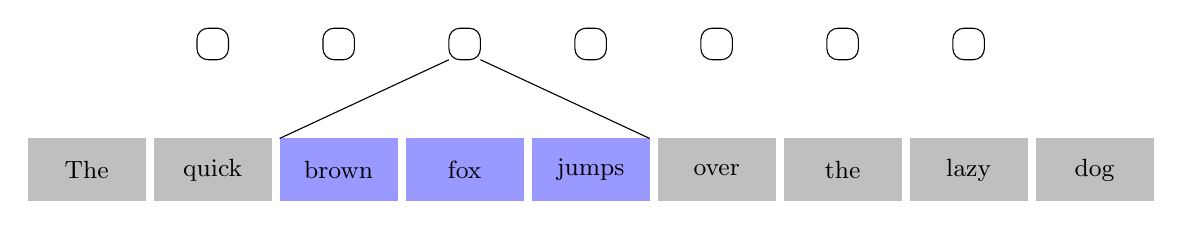
\begin{tikzpicture}[align=center, font=\small]

% Neurons
\draw[rounded corners] (-5, 1.4) rectangle (-4.6, 1.8);
\draw[rounded corners] (-3.4, 1.4) rectangle (-3, 1.8);
\draw[rounded corners] (-1.8, 1.4) rectangle (-1.4, 1.8);
\draw[rounded corners] (-0.2, 1.4) rectangle (0.2, 1.8);
\draw[rounded corners] (1.4, 1.4) rectangle (1.8, 1.8);
\draw[rounded corners] (3, 1.4) rectangle (3.4, 1.8);
\draw[rounded corners] (4.6, 1.4) rectangle (5, 1.8);

% Tokens
\node[fill={lightgray}, minimum width=1.5cm, minimum height=0.8cm] at (-6.4, 0) {The};
\node[fill={lightgray}, minimum width=1.5cm, minimum height=0.8cm] at (-4.8, 0) {quick};
\node[fill={blue!40}, minimum width=1.5cm, minimum height=0.8cm] at (-3.2, 0) {brown};
\node[fill={blue!40}, minimum width=1.5cm, minimum height=0.8cm] at (-1.6, 0) {fox};
\node[fill={blue!40}, minimum width=1.5cm, minimum height=0.8cm] at (0, 0) {jumps};
\node[fill={lightgray}, minimum width=1.5cm, minimum height=0.8cm] at (1.6, 0) {over};
\node[fill={lightgray}, minimum width=1.5cm, minimum height=0.8cm] at (3.2, 0) {the};
\node[fill={lightgray}, minimum width=1.5cm, minimum height=0.8cm] at (4.8, 0) {lazy};
\node[fill={lightgray}, minimum width=1.5cm, minimum height=0.8cm] at (6.4, 0) {dog};

% Arrows
\draw (-1.8, 1.4) -- (-3.95, 0.4);
\draw (-1.4, 1.4) -- (0.75, 0.4);

\end{tikzpicture}
\end{document}